\documentclass[12pt]{article}
\usepackage[english]{babel}

\usepackage{a4wide}   % A4 wide format
\usepackage{fancyhdr} % fancy header
\usepackage{graphicx} % graphics
\usepackage{setspace} % line spacing
\usepackage{subfig}
\usepackage{amsmath}
\usepackage{amsfonts}

\usepackage{natbib}
\bibliographystyle{apa}



%%%%%%%%%%%%%%%%%%%%%%%%%%%%%%
%% Dagger footnotes Definition %%
%%%%%%%%%%%%%%%%%%%%%%%%%%%%%%

\pagestyle{fancyplain}
\newcounter{daggerfootnote}
\newcommand*{\daggerfootnote}[1]{%
	\setcounter{daggerfootnote}{\value{footnote}}%
	\renewcommand*{\thefootnote}{\fnsymbol{footnote}}%
	\footnote[2]{#1}%
	\setcounter{footnote}{\value{daggerfootnote}}%
	\renewcommand*{\thefootnote}{\arabic{footnote}}%
}


%%%%%%%%%%%%%%%%%%%%%%%%%%%%%%%%%%%%%%%%%%%%%%%%%%%%%
%%  Definition of the paper title page             %%
%%%%%%%%%%%%%%%%%%%%%%%%%%%%%%%%%%%%%%%%%%%%%%%%%%%%%

\newcommand{\BMTitle}[5]{
	\thispagestyle{empty}
	%\vspace*{\stretch{1}}
	{\parindent0cm
		\rule{\linewidth}{.7ex}}
	\begin{flushright}
		
		% \vspace*{\stretch{1}}
		\sffamily\bfseries\Huge
		#1\\
		\vspace*{\stretch{0.5}}
		\sffamily\bfseries\large
		#2
		%\vspace*{\stretch{1}}
	\end{flushright}
	\rule{\linewidth}{.7ex}
	
	
\vspace*{\stretch{3}}
%	\begin{center}
%		\large #3 \\[1mm]
		
%		\vspace*{\stretch{1}}
%	\end{center}

\begin{tcolorbox}
	\begin{abstract}
		Adore Me is a U.S. lingerie e-commerce which heavily relies on data and technology to improve decision making and customer experience. It faces similar challenges as other fast fashion brands: short product lifecycles, long lead times, building an omnichannel experience, personalizing products and services, being effective in online and offline advertisement.
		
	 	Personalizing the customer experience and demand forecasting are some of the toughest and most rewarding challenges, which I takle using tools from Statistical and Machine Learning, Time Series and Bayesian Analysis. I present how these methods are used to recommend products, estimate churn and repurchase propensities and forecast the demand where traditional methods fail.
	 	
	 	While working on these models, I found that one cannot take them out of the organizational context and humans should be kept in the loop in order for these advanced algorithms to bring real value. The key factor is iteration and feedback, especially when even a simple, carefully designed model can be of great use to teams and in decision making.
		
		These models inform better decisions and help in automating heavy processes which are not easily treated with traditional software, but learned from data. \\
		


		\noindent \textbf{Keywords}: \textit{Demand Forecasting, Propensity Models, Fast-Fashion, e-commerce, Recommender Systems} \\
		\textbf{Acknowledgements:} \textit{Adore Me teams and people for continuous support, encouragement and learning opportunities during the last 3 years}
	\end{abstract}
	

\end{tcolorbox} 
%	\vspace*{\stretch{5}}
	
%	\begin{center}
%		\includegraphics[width=2in]{siegel}
%	\end{center}
    
	\vspace*{\stretch{1}}
	\begin{center}\sffamily\large{#5}\end{center}
	\newpage
	\thispagestyle{empty}
}
%%%%%%%%%%%%%%%%%%%%%%%%%%%%%%%%%%%%%%%%%%%%%%%%%%%%%

\pagestyle{fancyplain}
\lhead{}


% colors boxes and stuff
%%%%%%%%%%%%%%%%%%%%%%%%%%%%%%%%%%%%%%%%%%%%%%%%%%%%%
\usepackage{color}
\usepackage{tcolorbox}
\definecolor{light-gray}{gray}{0.95}
\tcbset{width=1\textwidth,boxrule=0pt,colback=light-gray,arc=0pt,auto outer arc,left=0pt,right=0pt,boxsep=5pt}
%%%%%%%%%%%%%%%%%%%%%%%%%%%%%%%%%%%%%%%%%%%%%%%%%%%%%

%%%%%%%%%%%%%%%%%%%%%%%%%%%%
%%  Begin the Document    %%
%%%%%%%%%%%%%%%%%%%%%%%%%%%%
\begin{document}
	


\BMTitle
{Data Science Applications at Adore Me:  \\
    a practice report}           % Title of the paper
{Mihai Bizovi \daggerfootnote{Senior Data Scientist (AdoreMe) | bizovim@gmail.com}
	} 
% First and Last name of authors
{12 May, 2019}                             % Geburtsort des Autors
{A project for the Logistics Course: \\
	
$\dagger$ Data Scientist (AdoreMe) | bizovim@gmail.com 
 }
{ASE, Cybernetics and Quantitative Economics, (May 2019)}  % Ort und Jahr der Erstellung
	
\newpage



\vspace*{-3cm}
\begin{figure}[!ht]
	\noindent\makebox[\textwidth]{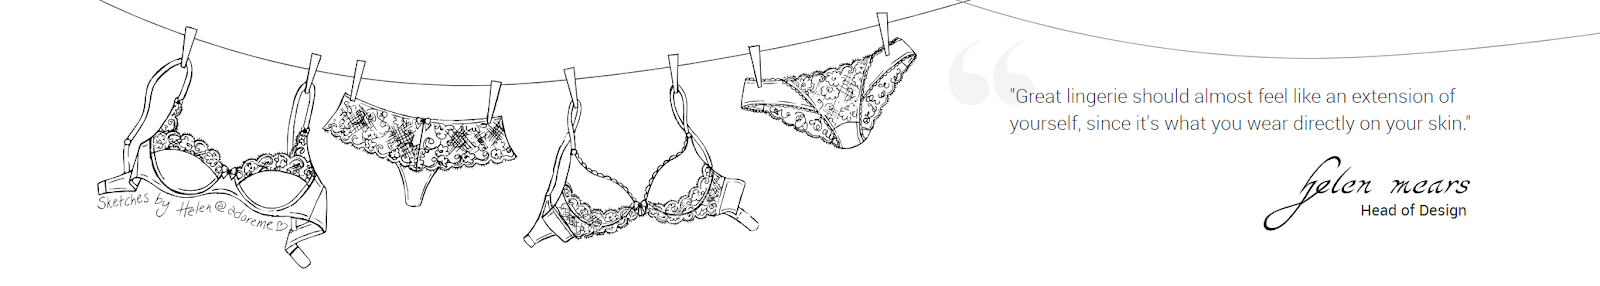
\includegraphics[width=\paperwidth]{graphics/helen.png}}
	\caption{Adore Me's mission is inspiring confidence, playfulness and making beautiful lingerie affordable to every type of body. \textit{(Source: adoreme.com \cite{adoreme})}}
\end{figure}



\tableofcontents

\newpage 

\listoffigures

\newpage


%%%%%%%%%%%%%%%%%%%%%%%%%%%%%%%%%%%%%%%%%%%%%%%%%%%%%
% Introduction %%%%%%%%%%%%%%%%%%%%%%%%%%%%%%%%%%%%%%
%%%%%%%%%%%%%%%%%%%%%%%%%%%%%%%%%%%%%%%%%%%%%%%%%%%%%
\onehalfspacing

\section{Introduction: Adore Me and the lingerie industry}

Adore Me INC. is a \textbf{lingerie e-commerce} operating in the U.S. and since the founding in 2012, became the second in market share, after Victoria's Secret. Although the gap is still very big, this shows how difficult it is to enter and survive in this niche market, as other players with similar evolution failed in the critical moments, mostly due to unsustainable growth inflated by funding rounds \cite{bankrupcies}. The company took opportunity left by competitors to enter the market as an e-commerce, which in time led to the technical expertise being one of the key drivers to success and scaling up.  %% Well, not only, but it is easier to get started online!!

\textbf{The message} of inspiring confidence, playfulness, being inclusive and making beautiful lingerie available for every kind of body at a reasonable price point resonated well with the diverse U.S. audience. The firm \textbf{grew exponentially} in the first years, driven by a \textbf{subscription-based} business model and effective TV advertisement. This introduced a set of challenges for the operations and supply chain.

Since then, Adore Me stabilized and consolidated as a middle-sized firm (around \$100 mln revenue), expanding beyond the subscription model towards the \textbf{omnichannel} experience, taking to account more ways customers prefer to shop for lingerie and personalizing the experience:

\begin{enumerate}
	\item \textbf{Pay as you go:} Shopping for products as in a typical e-commerce, although without the price cuts and benefits of the subscription.
	\item \textbf{Subscription:} The core business model, in which customers get a discount for items and every month they can either buy, accumulate store credits or skip the month(s) in order not to be charged. A lot of effort was put into making the communication of the terms as clear as possible and making the refunds easy.
	\item \textbf{Try before you buy:} The customer fills a quiz and receives a box with three items based on a Recommendation System, keeping what they like and fits, but returning the rest. It is suitable for customers who want to explore and try on more products and is by far the most challenging in terms of logistics and unit economics.
	\item \textbf{Retail:} Since October 2018, 4 stores opened inside malls in different locations along the East Coast. The idea is that weak malls are dying in the U.S., so it makes sense to compete with other brands in the strong ones. Moreover, the IT infrastructure in place allows customers to have a seamless experience between online and brick-and-mortar shopping. Despite the comparatively low volumes, it is a big challenge to scale towards many more stores across the country.
	\item \textbf{Marketplaces:} Integrating with marketplaces like Amazon offers new opportunities, but also risks, which are being mitigated by having a robust software architecture, easily extensible to such use-cases.
	\item \textbf{International:} Adore Me ships to Canada, Australia and plans to launch in UK and China in the future: a big challenge, since a lot of learning is needed in order to have success in those markets.
	\item \textbf{Brand spin-offs and Acquisitions:} Adore Me acquired \textbf{Bellabumbum}, a lingerie brand for expecting mothers. \textbf{Bijou} is the high-end line, emerging as a parallel brand.
\end{enumerate}

The following quotes give a sense of Adore Me's essence as an organization, which will be a key theme along the paper and helps to put the models and data in context.

\begin{tcolorbox}
	\begin{quotation}
		“The end goal is to craft the perfect bra and ship it to millions of women. So we’re talking about scalable e-commerce, coordinating our factories and robots in the distribution center, internal tools that catalyze everything.” | Adore Me \cite{adoreme}
	\end{quotation}
\end{tcolorbox}


\begin{tcolorbox}
	\begin{quotation}
		“Adore Me is the lingerie underdog, disrupting a huge traditional industry. We started the journey just 5 years ago and we’re one of the fastest growing companies in the US. The tech factor is strong in our DNA. We have more engineers than marketers, fashion designers or business folks and we’re proud of it.” | Adore Me, 2017 \cite{adoreme}
	\end{quotation}
\end{tcolorbox}



The competitive landscape is quite simple: The share of VS is estimated at around 54\%, and given the decreasing sales of ~\$8.5 bln worldwide, and the U.S. share is 70\%, the estimated U.S. revenue is around \$6 bln, all of that with 90k employees. Adore Me has 160 employees as of 2019 and \$105 mln in revenue, however just looking at these numbers doesn't do justice to the retail transformation that is happening lately and the pressure of changing customer preferences.

Even though buying lingerie online slowly becomes the new norm, brick and mortar stores are still essential for the customer experience and reach.

\begin{figure}[!ht]
	\centering
	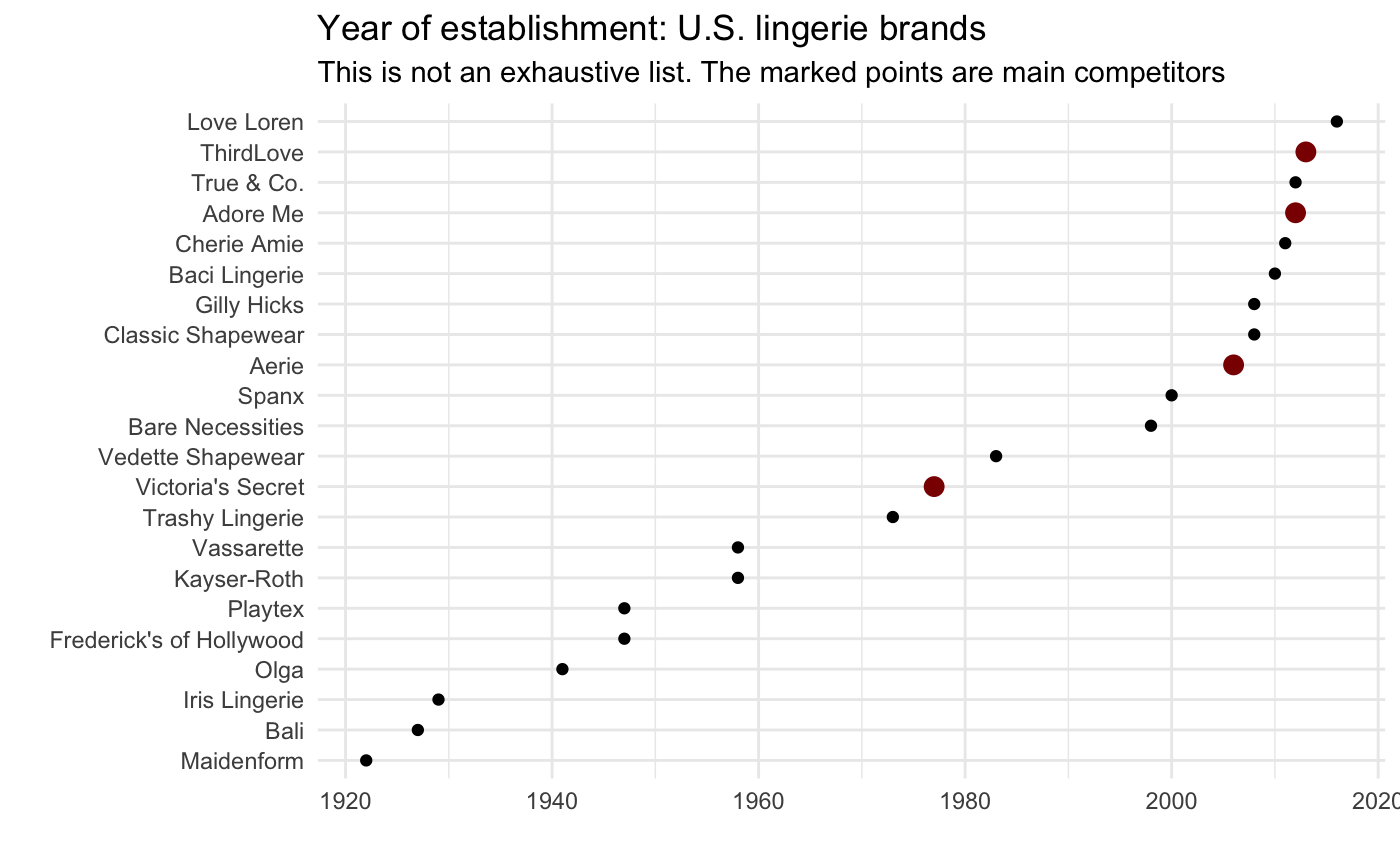
\includegraphics[width=0.8\textwidth]{graphics/us_firms.png}%
	\caption{U.S. lingerie firms and main competitors. It shows how hard it is to be relevant in this market dominated by VS. \\ \textit{\textbf{Source:} Wikipedia data, \textbf{Processing:} own design and crawling}}
\end{figure}


\subsection{Financial performance}

The purpose of this section is to highlight financial \textbf{features} of the business and determine the \textbf{parameters of analysis}. The secondary goal is starting to think in terms of unit economics. The company grew exponentially from 2012 until 2017 and then stabilized, improving the financial and operational health.

I take last three years of sales for the Subscription, PAYG purchases and plot the quantity of product sold. Decomposing the time series into Seasonal, Trend and Remainder gives great insight into the business mechanics: the biggest sales in a year are during Valentine's Day and Black Friday. Every month, the sales peak at its beginning, because customers have to make a decision regarding their membership: purchase, skip or unsubscribe. 

In contrast, every end of month has lowest sales. These fluctuations put pressures on the supply chain to be ready for a big amount of orders in a short time frame and plan the capacity accordingly. Good news is that the patterns are regular, and remainder can be explained by other factors. An important take away is that seemingly unrelated teams, Marketing and Supply Chain should collaborate closely to take into account these trends in replenishment and purchasing decisions.

\begin{figure}[!ht]
	\centering
	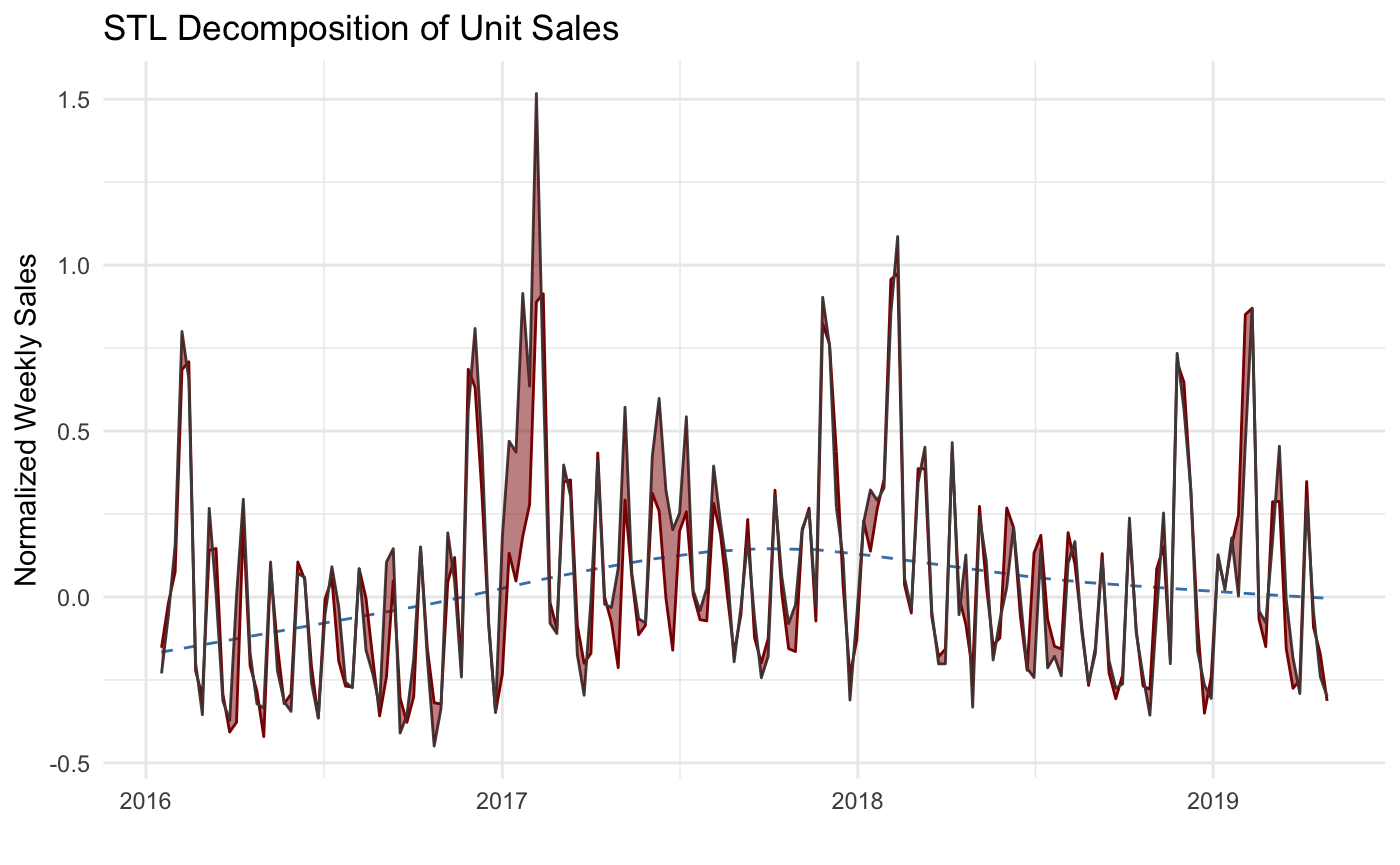
\includegraphics[width=0.8\textwidth]{graphics/stl_sales.png}%
	\caption{STL Decomposition of the evolution of sales (on a relative scale), transformed by the Box-Cox with optimal $\lambda$.  \\
		\textit{\textbf{Data Source:} Adore Me, \textbf{Processing:} Own processing and design}}
\end{figure}

The dashed blue line is estimated trend and red shaded areas the remainder of decomposition. The dampened trend is due to a part of customers converting to Try Before you Buy (Elite). The dynamic goes as follows: sales are driven by new and existing customers, which in turn is driven by the marketing budget and conversion rates.
%ACtivity profile, size, complexity, financial, etc



\subsection{Organizational Culture and Values}

Teams at Adore Me are small, self-organized (4-6 people) and the organizational structure is non-hierarchical. The philosophy and ``modus operandi`` is greatly inspired from Agile and Kaisen methodologies, with an emphasis on fast iteration, continuous improvement and learning. This is especially true for technical and engineering teams, who strive for automation, but leave space for the human touch and creativity.

Thus, we can view the processes as networks of interaction and collaboration between different teams, who try to improve and adapt fast to the changing realities. Another unusual feature is that the business (NY) and engineering (Bucharest) work closely to build tools and software that crystalizes and automates processes, facilitates communication, improves decision making using data, statistics, machine learning and optimization. This internalization of tools and processes is in stark contrast with the current trend of IT externalization and heavy use of consultants. 

The fact of being an Agile hybrid tech and lingerie company enables Adore Me to be customer-centric, heavily use data for decision-making, iterate fast. Being the closest to problem, teams can be very efficient and creative. This is a decentralized way of dealing with dynamic complexity, relying on the underlying processes, informational/software ecosystem and human competence.

\begin{figure}[!ht]
	\centering
	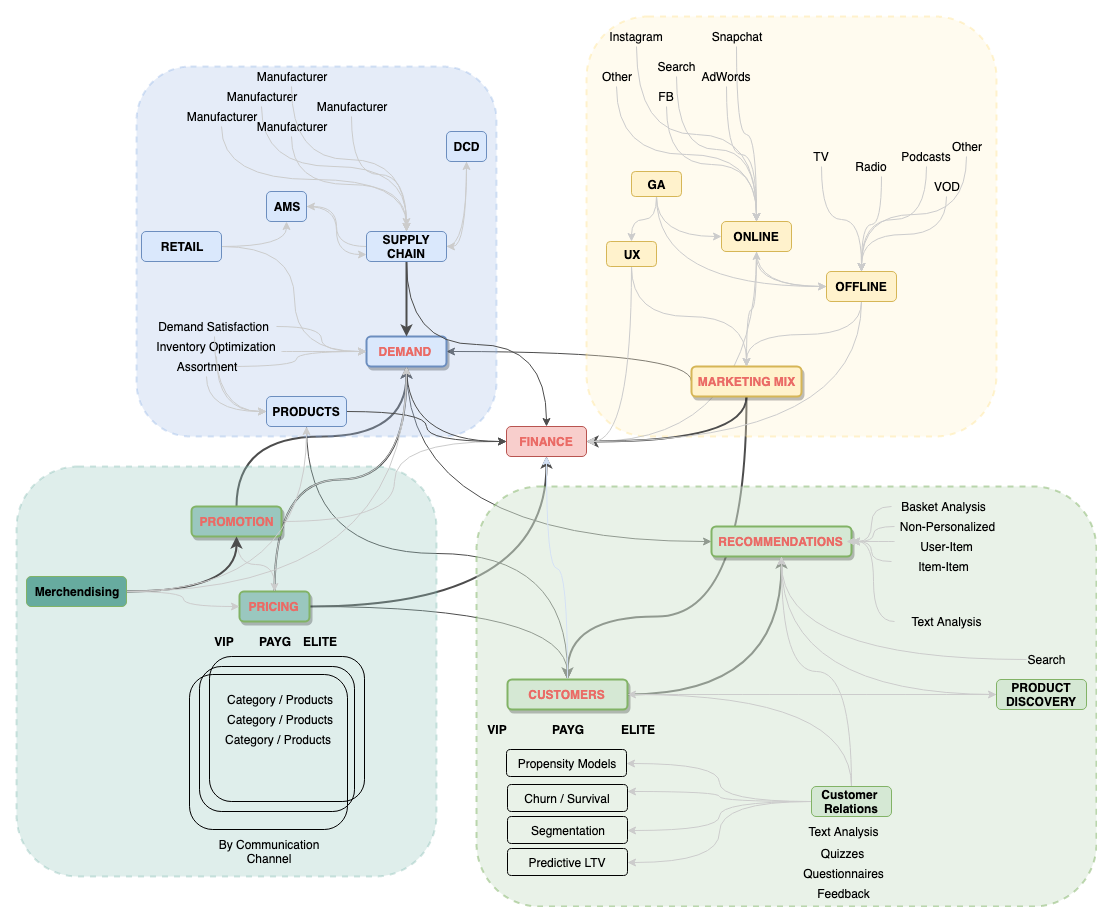
\includegraphics[width=1\textwidth]{graphics/conceptual_map.png}%
	\caption{A map of challenges at Adore Me, handled by self-organized teams.  \\
		\textit{\textbf{Source:} Own Design}}
\end{figure}


The map above shows that in this kind of e-commerce, marketing and merchandising decisions impact the supply chain operations more than one would expect, a fact made even more visible by the obvious seasonality. In order to understand those features, a discussion around  internalization, externalization, software architecture and various integrations is needed. 



\subsection{Data and BI team}

Data and BI is a team of 5 people responsible for capturing data at scale across multiple ecosystems and leverage it in order to improve decision-making and bring value. I am the Data Scientist, solving business challenges in marketing, engagement and supply chain as well as developing the infrastructure for statistical and machine learning modeling, data pipelines and decision support applications. The team works according to Agile methodologies, is self-organized and cross functional, as it is well versed in data pipelines, warehousing and databases, BI and programming. 

In this project I will focus on the analysis and modeling aspects of the work, but it implies the full range of building end-to-end systems: from problem formulation, to data collection and model operationalization. A nice tool before starting any project, is the hierarchy of analytic needs, proposed by Google, which emphasizes the need to start simple and grow the complexity along with the maturity and needs. There are several levels in the hierarchy, starting from the most basic level, which helps to avoid cracking a nut with a sledgehammer.

\begin{figure}[!ht]
	\centering
	\includegraphics[width=0.45\textwidth]{hierarchy.png}%
	\caption{A subjective view of the level in hierarchy different projects at Adore Me are at. By expanding the area of competence within and between applications, we share know-how and bring value faster. \\
		\textit{\textbf{Source:} Own design and processing}}
\end{figure}

As of today, we're making rapid progress in demand forecasting, recommender systems and engagement using cutting edge techiques and models which are appropriate for the challenges faced. This frees teams from some of the cognitive load caused by repetitive tasks and allows to search for even more creative solutions.

\begin{enumerate}
	\item The drawing board: domain understanding, problem formulation, collaboration
	\item Establishing processes, learning and exploration
	\item Crystalizing processes into software products and data collection
	\item BI, Controlled experiments and Statistical Models 
	\item Machine Learning, Optimization, Bayesian Methods
\end{enumerate}

The toolbox at top of hierarchy frees up time to focus on the creative part of the job. In order for models, e.g. in demand forecasting to bring real value, a team usually has to go through all of these stages. In terms of technological stack, we heavily use tools from the Google Cloud Platform and define everything in terms of code, for maximum automation and reproducibility, both in data warehousing and machine learning.

\begin{figure}[!ht]
	\flushleft
	\includegraphics[width=0.9\textwidth]{project_outline.png}%
	\caption{Data flows for Data Warehousing, using a Google Cloud Platform technological stack consisting of Virtual Machines, Containers, Batch and Streaming Pipelines, Queues.  \\
		\textit{\textbf{Source:} Horia Niculescu, Joint presentation with Bizovi Mihai at Google DevFest}}
\end{figure}



\section{Recommender Systems}

Adore Me sells bras, lingerie, sleepwear and activewear of own design in a wide range of sizes (30A-46DDD, XS-4X) through multiple business models. Because of the subscription service, Adore Me has a themed showroom with new products every month, which means that robust processes are needed in order to bring a product to market: from the idea, design, manufacturing to making it available for orders. 

Besides new products and the overall short life cycle, procurement and supply chain teams have to make hard decisions on what product to replenish, discontinue, what quantity of each size needs to be manufactured in order to satisfy the customer demand. This process of bringing a product to market involves a lot of teams that need to collaborate: procurement, logistics, finance, marketing and merchandising, all with the support of IT tools developed in house. 




\begin{figure}[ht!]%
	\centering
	\subfloat[bras and panties]{{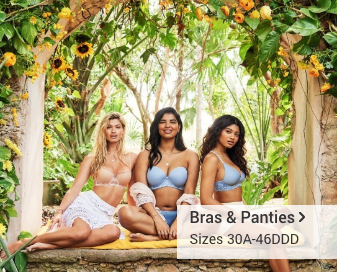
\includegraphics[width=7cm]{graphics/bras.png} }}%
	\qquad
	\subfloat[swimwear]{{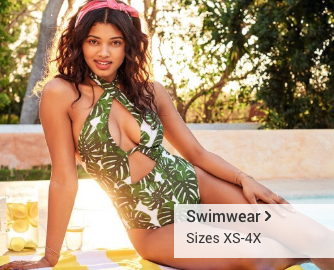
\includegraphics[width=7cm]{graphics/swimwear.png} }}%
	\caption{An example of a themed ``showroom`` for May 2019. An important aspect is the large size range, which makes the demand forecasting to be of tremendous importance \\
		\textit{\textbf{Source:} Screenshot from adoreme.com}}
	\label{fig:example}%
\end{figure}


Another important aspect of the way Adore Me sells products is the concept of sets: matching tops (bras) and bottoms (panties). I introduce the sizing matrix, which is an essential instrument, both for customers to choose the right one and for Adore Me to make good decisions regarding their availability. When building recommender systems, one cannot rely solely on Collaborative Filtering, both because of data limitation (most customers have purchased only few products) and business specifics. This means that the algorithms used should take into account information about customers and products.


\begin{figure}[!ht]
	\centering
	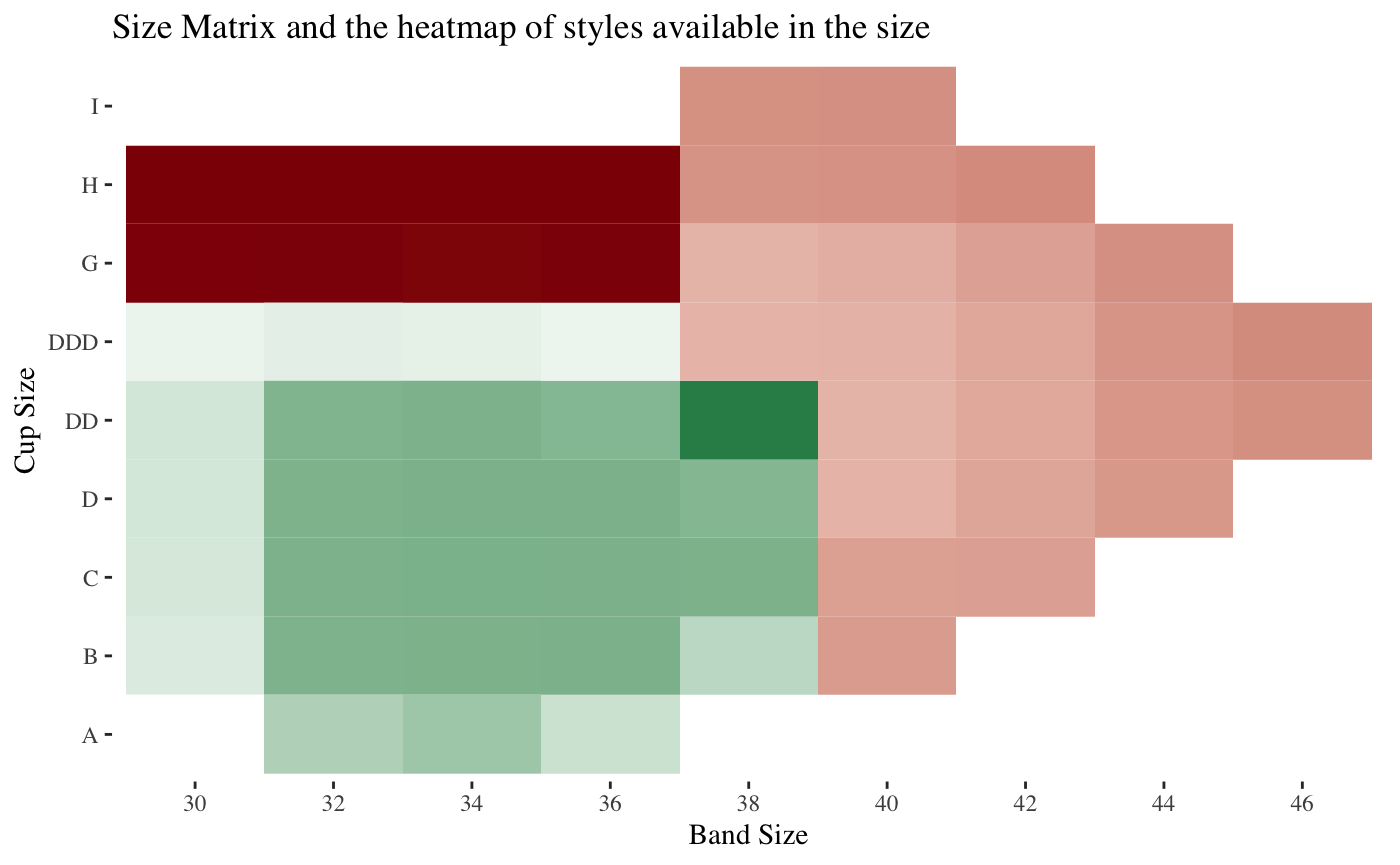
\includegraphics[width=0.7\textwidth]{graphics/size_breakdown.png}%
	\caption{Anonimized size matrix for the products available on the website. \\
		\textit{\textbf{Data Source:} Adore Me, \textbf{Processing}: Own design and processing}}
\end{figure}


\subsection{Content-Based Filtering}

Customers have heterogeneous preferences in styles, colors, product types and sizes. Even though an e-commerce has a large catalog of products, customers hardly scroll past the first page in order to find ``the product``. This is why recommender systems are essential for this kind of e-commerce: to suggest products that a customer might like, in the right size availability, season and close to their preference. There is also an element of serendipity, where customers discover unexpected styles, which are intriguing but never thought about them before.


The traditional way of doing merchandising is hitting its limitations of what it can achieve in terms of product discovery. A big part of inventory management is the story between slow and fast moving items, so there is a component of an inherent/latent product popularity and customer preferences. A long tail of slow-moving items is problematic for replenishment, reason why a careful analysis is needed in order to reduce the number of products, keep the best, while not sacrificing much from customers' choice.

This variety, combined with short lifecycle of products, if is not managed well, can cause cannibalization between products and saturation of categories. It is also important to note that preferences of new and existing customers, in retail versus online differ significantly. A product which is a bestseller on the website might not work well in a store. The dynamics of e-commerce products is governed by the ``laws of large numbers``, while there is much more uncertainty in the retail world.

\begin{figure}[!ht]
	\flushleft
	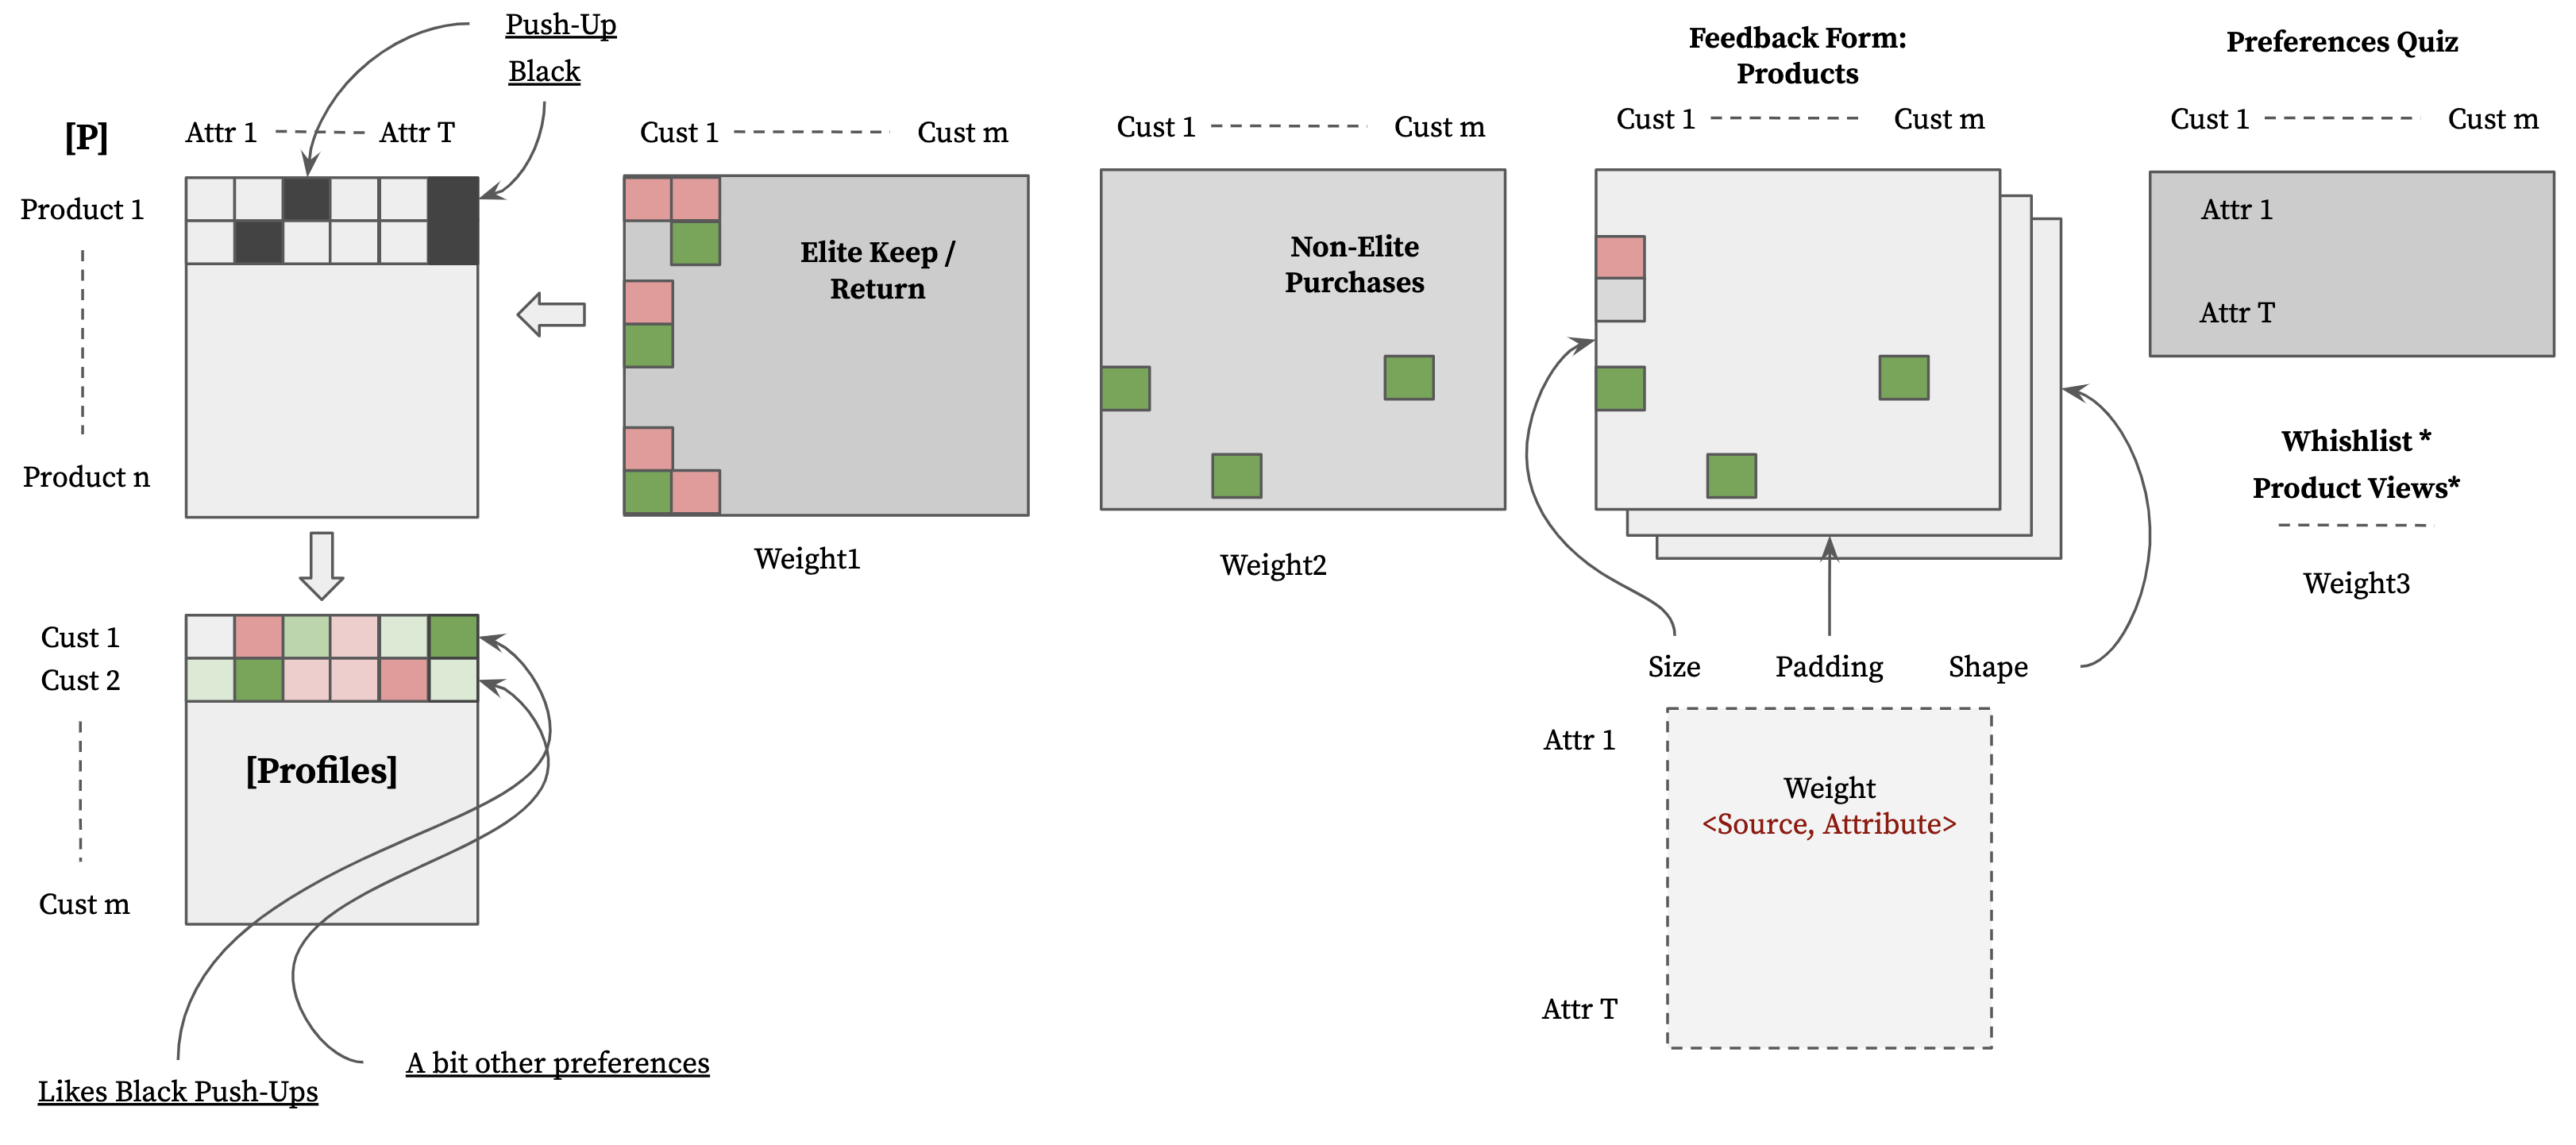
\includegraphics[width=1.1\textwidth]{graphics/elite_recommender.png}%
	\caption{An example of Content-Based Recommender System, which can give great insight into customer preferences and deal with some challenges of personalization.  \\
		\textit{\textbf{Source:} Own Design and Model}}
\end{figure}

The content-based filtering I built makes use of the quizzes customers fill in at registration, regarding some of their preferences and sizes, feedback given for products in terms of fit, quality and styles, purchases and returns among different channels, views, add to cart of products and a database of carefully curated product attributes.

As presented in \textit{(Figure 9)}, the key component is deriving a matrix of customer profiles, where an observation/row represents customer preferences of different product attributes. This profile matrix is a weighted combination of the previously described sources, where a score is given to positive/negative actions, thus the attributes are penalized or reinforced. Let $\mathbf{R}^a_f$ be the "rating" matrix given to various product attributes, where the superscript refers to fit, style and fit. A weight is given for each source and attribute. $\mathbf{R}_q$ gives the preference from customer quizzes, $\mathbf{R}^c_p$ from customer purchases and returns among different channels and $\mathbf{Q}$ the one-hot-encoded matrix of product attributes.

\begin{equation}
	\mathbf{P} = \mathbf{Q} \cdot \big( w_p  \mathbf{R}_p + w_f \mathbf{R}_p + w_q \mathbf{R}_q  \big)
\end{equation}

Each signal source is given a weight, as well as each attribute, which is informed by business knowledge and optimized to maximize the probability of a customer purchasing it. The resulting matrix of profiles $\mathbf{P}$ is a representation of their preferences.


\subsection{Association Rule Mining}

This method takes into account a lot of information, but sometimes we want to see what products are often purchased together, in order to display recommendation under a product page, with an explanation of "customers who bought this also bought the following products". Association rule mining is a classical algorithm which mines a transactional database of orders/baskets for products which are often bought together and their relationship is statistically significant.

I use an own, scalable implementation of Apriori algorithm to derive important rules of the form $\{ p_1, p_2 \} \implies \{ p_n \}$, which can be used for merchandising decisions and recommendations. The rules are assessed according to the support (frequency of appearance in the database), confidence and lift (how more likely are the products bought together relative to the case if they were independent). An important limitation of the method is that it doesn't tell a causal story, but is useful enough in order to suggest improvements for the merchandising team.

\begin{figure}[!ht]
	\centering
	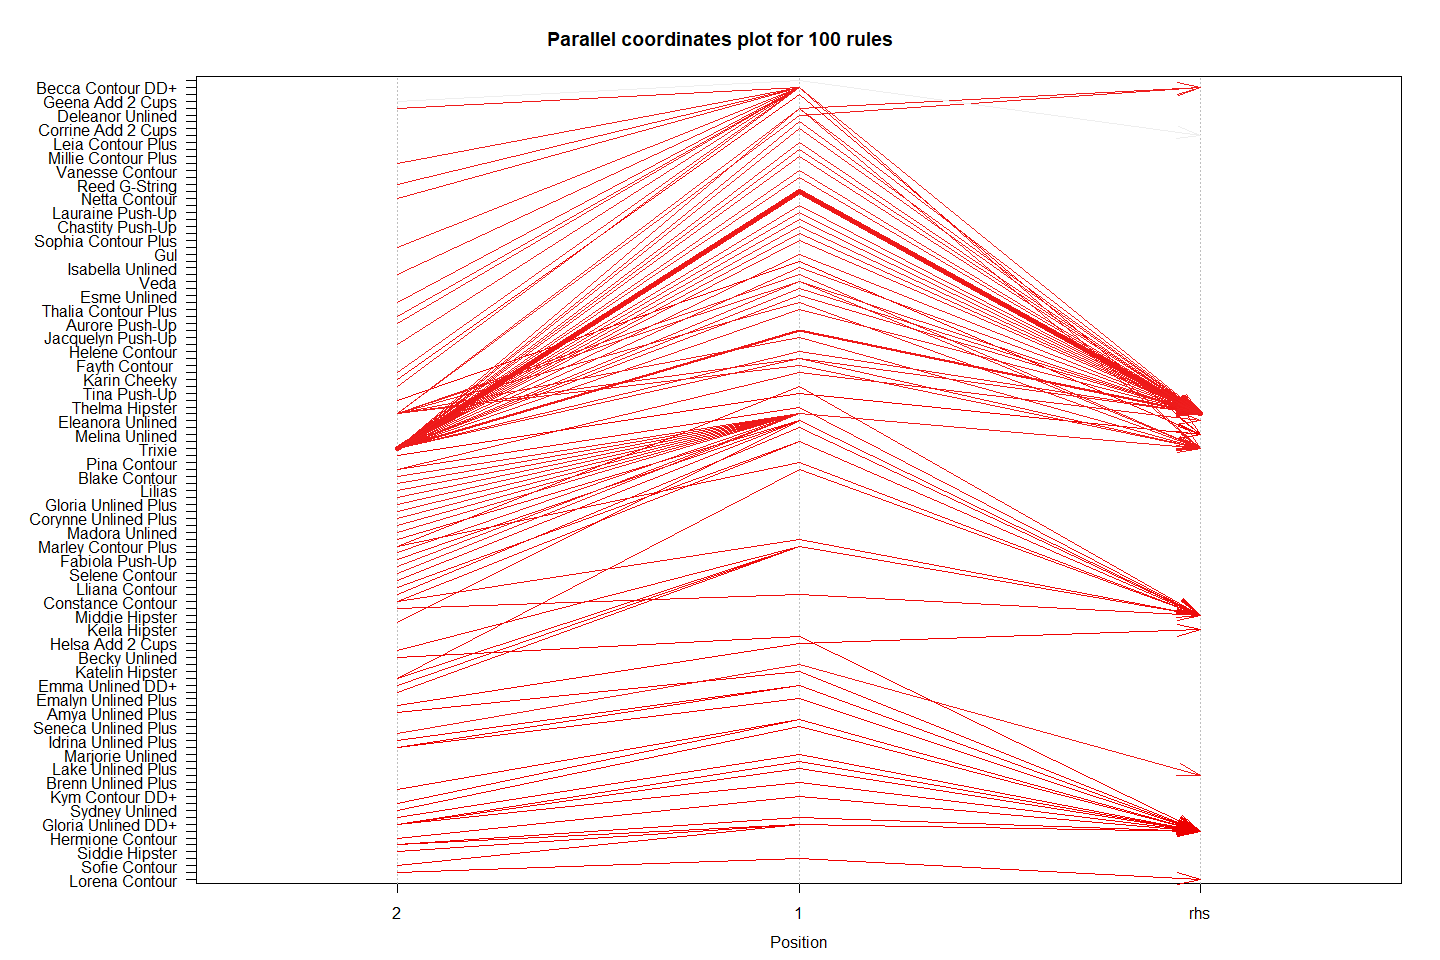
\includegraphics[width=1\textwidth]{arules.png}%
	\caption{A parallel coordinates plot to visually investigate items bought together  \\
		\textit{\textbf{Data Source:} Adore Me \textbf{Processing:} Own processing and design}}
\end{figure}


\section{Propensity Models}

In order to limit the scope of this project, I choose to focus on propensity models of churn and repurchase over marketing mix and attribution modeling, which are also very exciting applications. Having a large, heterogeneous user base poses a challenge to engagement teams of who to target, with what communications, offers and over what channels in order to maximize their lifetime value relative to the "investment".

Rule-based systems and targeting have their limitations in capturing this heterogeneity and having a predictive power over what the customer is likely to do next. This is where machine learning and statistical methods shine, by taking into account a large range of customer attributes, purchasing patterns and even their product preferences. The model learns on historical data, and after a careful validation of the model (cross-validation in time) and when we made sure the model performs well without "peeking" into the future, we use it to score the customers and design experiments to measure the uplift of engagement campaigns. 


\subsection{Churn}


A simple A/B test doesn't take into account the difference between customers with a "high" and "low" score, in terms of what would happen if they were not targeted. We follow the methodology outlined by Eva Ascarza in order to measure the uplift:

\begin{itemize}
	\item Leave out an overall control group.
	\item Select a random sample of customers and split them in control and target groups.
	\item Select another sample according to repurchase or churn propensity: split in control and target groups.
	\item Measure the uplift in sales and margins.
\end{itemize}

Applying machine learning models is more complicated than it looks, because we have to make sure it generalizes over next intervals of time, fix imbalances in class distributions, score all customers and decide on the trade-off between precision and recall. Moreover, the churn/unsubscription dynamics are very different from traditional applications of these models in telekom and gaming industries, so the question is what can be done about it. In our case, is mostly by improving the service, delivery, having better products in customer' sizes and making the user experience in exchanges/returns easier. Even if a model can predict very well the churn probability, it is hard to find an obvious action to rectify it. However, these models have a great success in repurchase, which informs after a careful data analysis strategies for targeting, offers and personalized recommendations.

I use boosted trees (XGBoost), survival and probabilistic models in contractual settings, as the event of churn is well defined. The problem is more challenging in Pay as you go, as the event of becoming inactive is latent, unobservable, but can be inferred from data.

\subsection{Repurchase}

A graphical representation of the problem is best represented by the following plot, where each row is a customer and points are purchases. For the churn model, the events can be of a different type: skip, unsubscription or purchase. We can see the heterogeneity in customers and their purchasing habits in terms of frequency, recency and revenue.  

\begin{figure}[!ht]
	\centering
	\includegraphics[width=0.7\textwidth]{payg_patterns.png}%
	\caption{Purchasing patterns for a sample of PAYG customers.  At a certain point, we want to estimate the probability of repurchase during a forecasting horizon.\\
		\textit{\textbf{Data Source:} Adore Me, \textbf{Processing:} Own design and processing}}
\end{figure}




\section{Demand Forecasting}

The specifics of fast-fashion industry make demand forecasting a very hard task, as we cannot possibly take all factors into account: did the product appear in an advertisement, was it placed very high on the website, did customers like the picture of model, was the marketing budget unexpectedly increased or decreased? This is why the classical ARIMA, ETS and time series analysis \textbf{alone}, are often inadequate for the patterns we observe, thus, also the assumptions of EOQ-like models break down miserably, and we have to resort to simulation and optimization techniques, Bayesian statistics and machine learning.


\textbf{If that wasn't enough, going omnichannel} and opening new stores makes matters even ``worse``, as they have a different dynamic, time frames and feedback loops. When we make a decision to order from manufacturers a certain quantity of products, we should at least take into account interactions between these channels. Just aggregating the data would wash/cancel out important patterns, which are critical for good decisions of distributing products across channels.

The goal of this section is to introduce and develop forecasting modeling techniques that are appropriate for the fast-fashion industry. I already outlined and presented the challenges that I intent to tackle, from short product lifecycles, variety and hierarchies, sizing and the omnichannel experience. Most of the traditional literature in Supply Chain Management uses analytic techniques, MOQ-related models and classical time series analysis. While it might work well for certain use cases, as there are definitely providers of such analytic software, it solves a very small subset of problems Adore Me is facing, for well defined patterns at style level.

In this project, I forecast at style level and use the concept of size breakdown, in order to distribute the quantity to sizes, a pattern which is remarkably stable among several product and body types. This approach to modeling, however, doesn't take into consideration how the dynamics of size depletion influences customer behavior on the website, which in turn heavily influences sales. In a nutshell, the costs to forecasting mistakes are: 

\begin{itemize}
	\item In the case of under prediction, the team buys less inventory and the products go out of stock, so there is a lost sales opportunity and some customer dissatisfaction that a product they really like is not available in their size.
	\item Being too optimistic about products' expected demand, leads to excess inventory and investment which could be put to a productive use. It can also lead to distruptive imbalances in inventory structure
\end{itemize}

Sometimes, it is impossible to foresee the success of some products, which become wildly popular or predict the under performance of seemingly promising one. A good example is ``Gynger``, as every year at VDay, no matter how aggressively we procure, it goes out of stock. This means there are certain things beyond our control or cognitive abilities, and we cannot foresee or capture all factors, but we can do better in the majority of cases. I provide examples of product sales, the challenges in forecasting and propose methods that are promising in particular situations: for new products, short and long history. The key difference is that these (machine learning and Bayesian) modeling techniques allow to incorporate domain knowledge and learn/update key parameters from data. These models have great representational power and are flexible, but useless if the problem is not well formulated or if there is no pattern in the data. This is why a critical component to good forecasting is having well designed features.

An important requirement for the forecasting methods is for them to be automated, as it is not reasonable to tune and check manually hundreds of models every two weeks. This said, it doesn't mean that it replaces humans, on the contrary, these results should be ``explainable``, which might be hard with some machine learning methods, but not impossible. The philosophy is to give reasonable and interpretable defaults, which can be challenged in the whole process.

%%%%%%%%%%%%%%%%%%%%%%%%%%%%%%%%%%%%%%%%%%%%%%%%%%%%%
\subsection{Forecasting New Products and the Product Lifecycle}

Forecasting the demand for new products is an interesting research topic of tremendous practical importance, in which the focus has mostly been on diffusion models. The problem is that you need at least 3 data points in order to generate the forecast. But in practice, the situation is even worse: how do you forecast a new product half a year in advance? It would be great if we could base the forecast on product attributes and seasonality, define some methodology and iterate on it. Unfortunately, there is much more nuance to the problem, as the naive approach is not enough: it doesn't generalize well.


The key is enriching the ``training`` data with meaningful features, which leverage similarity between products, seasonality, extracts sales patterns from groups of attributes. It uses a clustering and similarity module in order to identify similar products according to their functionality, attributes and even look (if using images). Finding products with similar launch sales patterns (in terms of shape, invariant to shifts, translations and distortions) turns out to be a valuable exercise when connected with product attributes. This fact can be use to create clusters of products which would bring more information for the item being forecasted. If products which have nothing in common get into the same cluster, it might be a statistical coincidence, quirk of the model, or more interestingly, those products might be influenced by other drivers.

There are three non mutually exclusive ways of doing such clustering: based on attributes (even text descriptions and images), extracting features from time series (trend, curvature, ACF, seasonality, entropy, perceptual importance points) and using a specialized distance metric like \textbf{Dynamic Time Wrapping} or Cross-Correlation on raw or normalized time series.


\begin{figure}[ht!]%
	\centering
	\subfloat[perceptual importance points]{{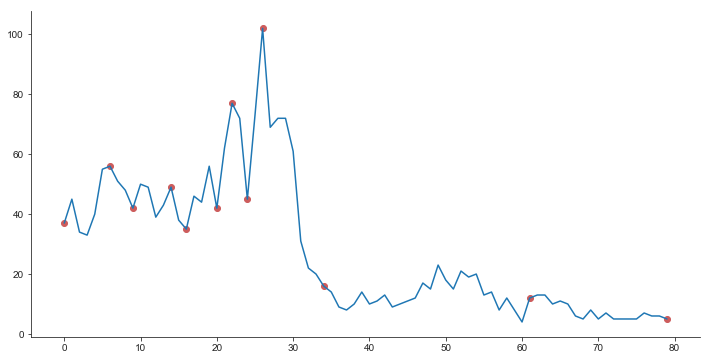
\includegraphics[width=8cm]{graphics/001.png} }}%
	\qquad
	\subfloat[dynamic time wrapping neighbor]{{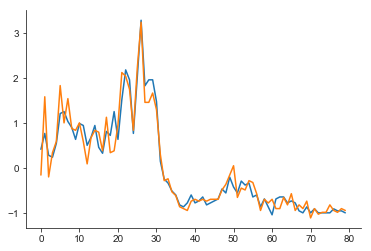
\includegraphics[width=6cm]{graphics/004.png} }}%
	\caption{An example of using \textbf{Perceptual Importance Points} applied on a launch pattern of a new products.\\
		\textit{\textbf{Data:} Adore Me, \textbf{Processing:} Own processing and design}}
	\label{fig:pip}%
\end{figure}

A method to reduce the dimensionality of time series for clustering is on the left plot. On the right is the result of finding the nearest neighbor using Dynamic Time Wrapping Nearest Neighbor search. The products have sales of different magnitudes because of color, but the underlying pattern similarity is striking. 


Before moving to the actual forecasting methods, it is important to have in place a validation procedure, in order to test the performance of several models. The business process guides this design: I use historical data to train a model, then make predictions during validation and launch. Since we go back in history, we know what actually happened and can benchmark a new model against an old one or human experts. Choosing the model based only on fit or backtesting is a questionable practice, with which we cannot get away in the current setting.

\begin{figure}[!ht]
	\centering
	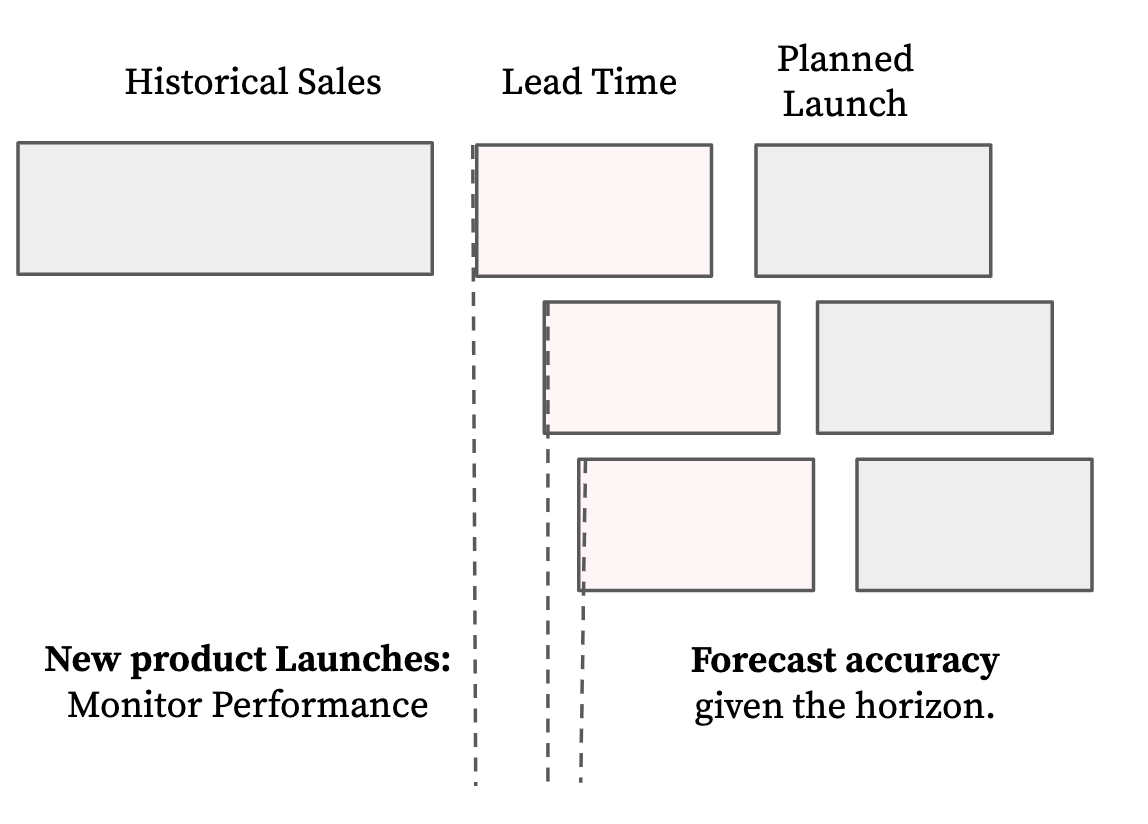
\includegraphics[width=0.5\textwidth]{graphics/validation_strategy.png}%
	\caption{The training | validation | test split, which can be used to prove the added value of models to the Demand Forecasting and Management. Comparing forecasts with actual sales, inventory evolution we can quantify (in \$) how much we gain from an improvement in forecast accuracy. \\
		\textit{\textbf{Design:} Own design}}
\end{figure}

I focus on two classes of models which are suitable for combining information from multiple sources and capturing complex interactions between latent properties of a product, seasonality and business trends. The first one, described in the next page is a hybrid Recurrent Neural Network with LSTM units on the left branch and a Feed-Forward Neural Network with Embeddings on the right. The problem is modeled as a sequence prediction and uses as inputs all drivers we discussed until now. The problem is that such models are very hard to train, a reason we might use simpler models (in terms of representational power), but which are more practical and interpretable: Bayesian Hierarchical Models, which leverages variance pooling to estimate the parameters at group and population level. Why Bayesian and not classical models on panel data? Because of the big amount of parameters and lack of information, because of the ability to introduce expert knowledge in prior distributions and update those parameters continually, as we get more data.

\begin{figure}[!ht]
	\centering
	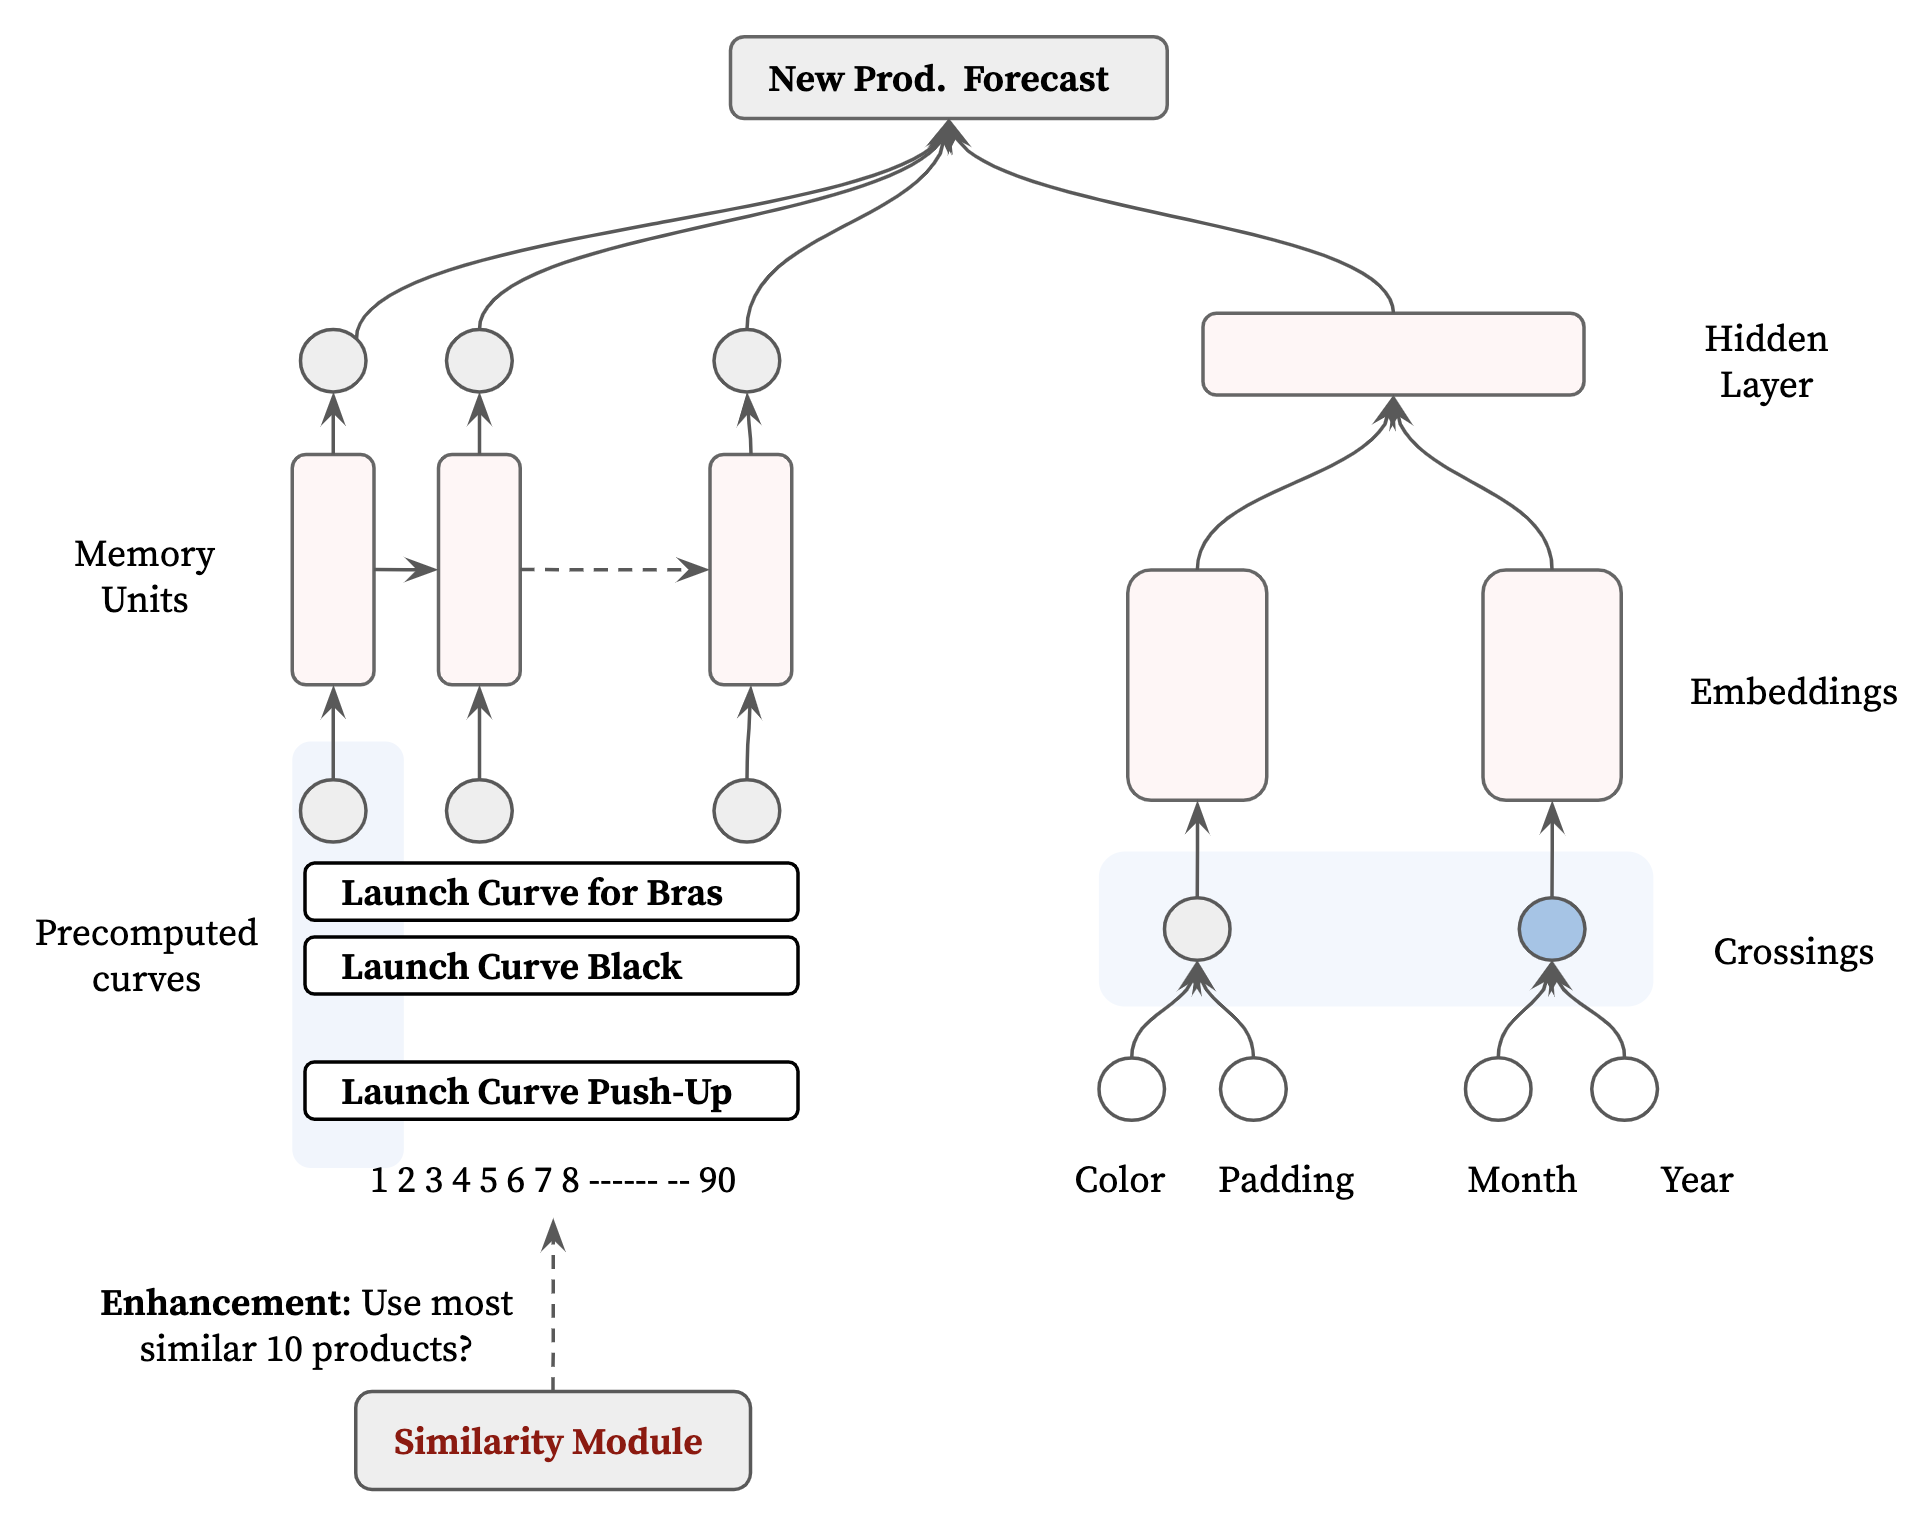
\includegraphics[width=0.7\textwidth]{graphics/LSTM_architecture.png}%
	\caption{A hybrid LSTM and Embedding FFNN Architecture. It captures the most important factors which drive the variance in product sales. \\
		\textit{\textbf{Source:} Own Design and Architecture}}
\end{figure}

\begin{figure}[!ht]
	\centering
	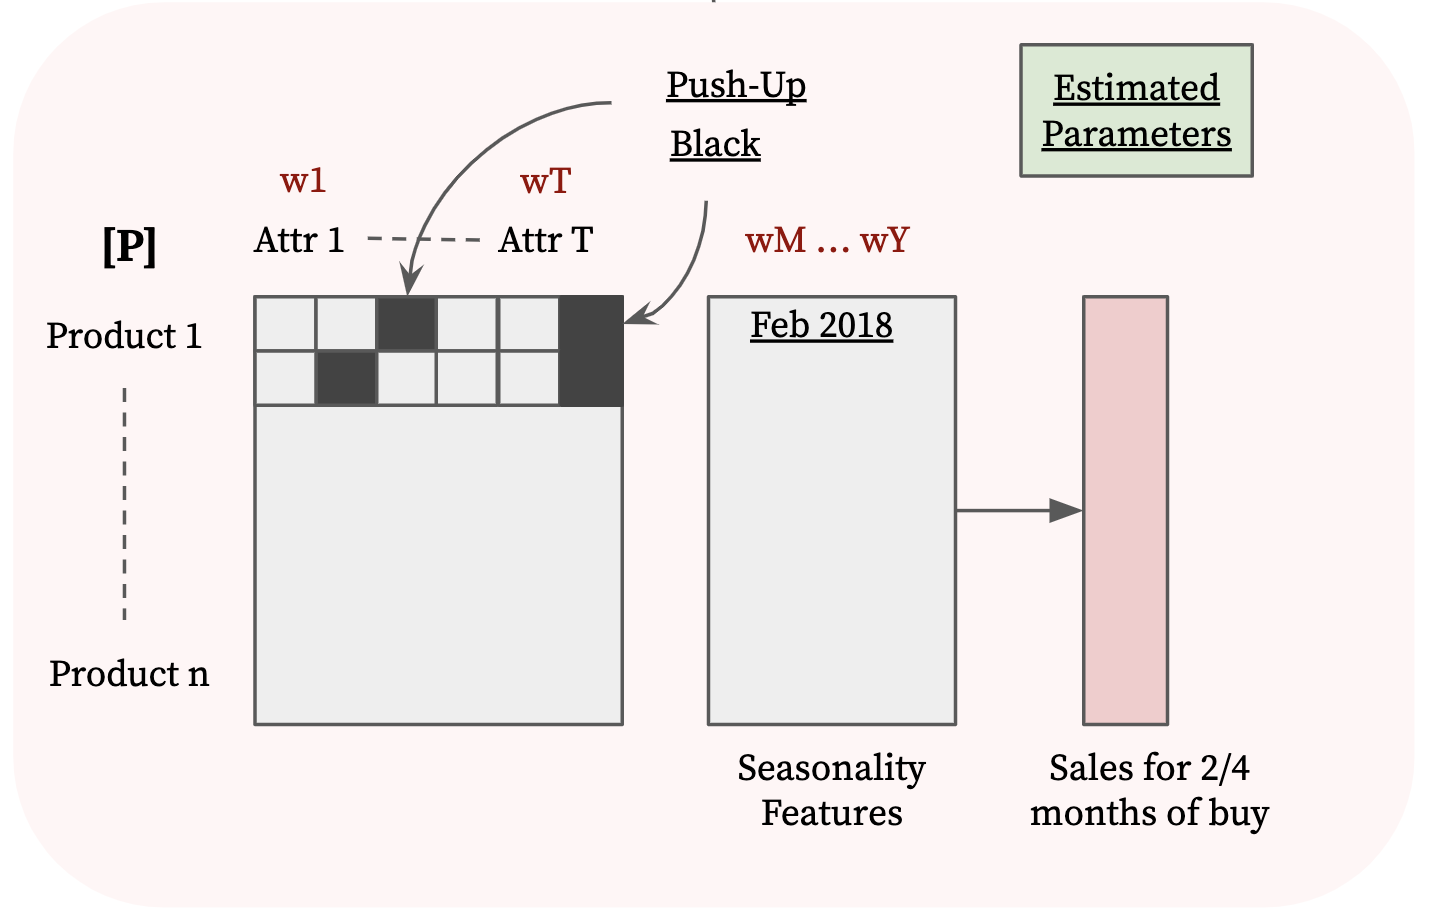
\includegraphics[width=0.7\textwidth]{graphics/regression.png}%
	\caption{A snapshot from the panel training data for a Bayesian Hierarchical Model. The concept is very similar to the neural network above, but the approach is probabilistic from end-to-end. At style level, it would be a 3D tensor and 4D at size level. \\
		\textit{\textbf{Source:} Own Design and Architecture}}
\end{figure}


%%%%%%%%%%%%%%%%%%%%%%%%%%%%%%%%%%%%%%%%%%%%%%%%%%%%%
\subsection{Forecasting Short History Products}

All the tools gathered in previous section directly translate to forecasting products with a short history, with the remark that in this spot I have more literature to draw ideas from, including a brilliant thesis by [4] and article in Intelligent Fashion Forecasting [5].

An important feature of short time series, is that I can't extract the seasonality with STL or methods that require two full periods. This leaves us with the same set of creative techniques to be leveraged here. Another question might arise: \textbf{why working with daily data} and not weekly or monthly, as the latter would result in much smoother pattern. The answer is that it depends on the situation and know how. The company was using data at a higher level of aggregation in order for the classical methods not to break down and generate wild forecasts. However, it loses important information and patterns, which can be leveraged with other approaches. The same holds true to size-level forecasts versus size breakdown matrices: it all depends on the use-case and capabilities/maturity of people doing forecasts, and building forecasting software.

From the plots below, we are clearly dealing with multiple seasonalities and need to decide what to do with out of stock time periods. Do we ignore it, replace with a counterfactual (what would've happened if it were available), interpolate? These are hard questions which depend on the modeling approach and objectives.

\begin{figure}[!ht]
	\centering
	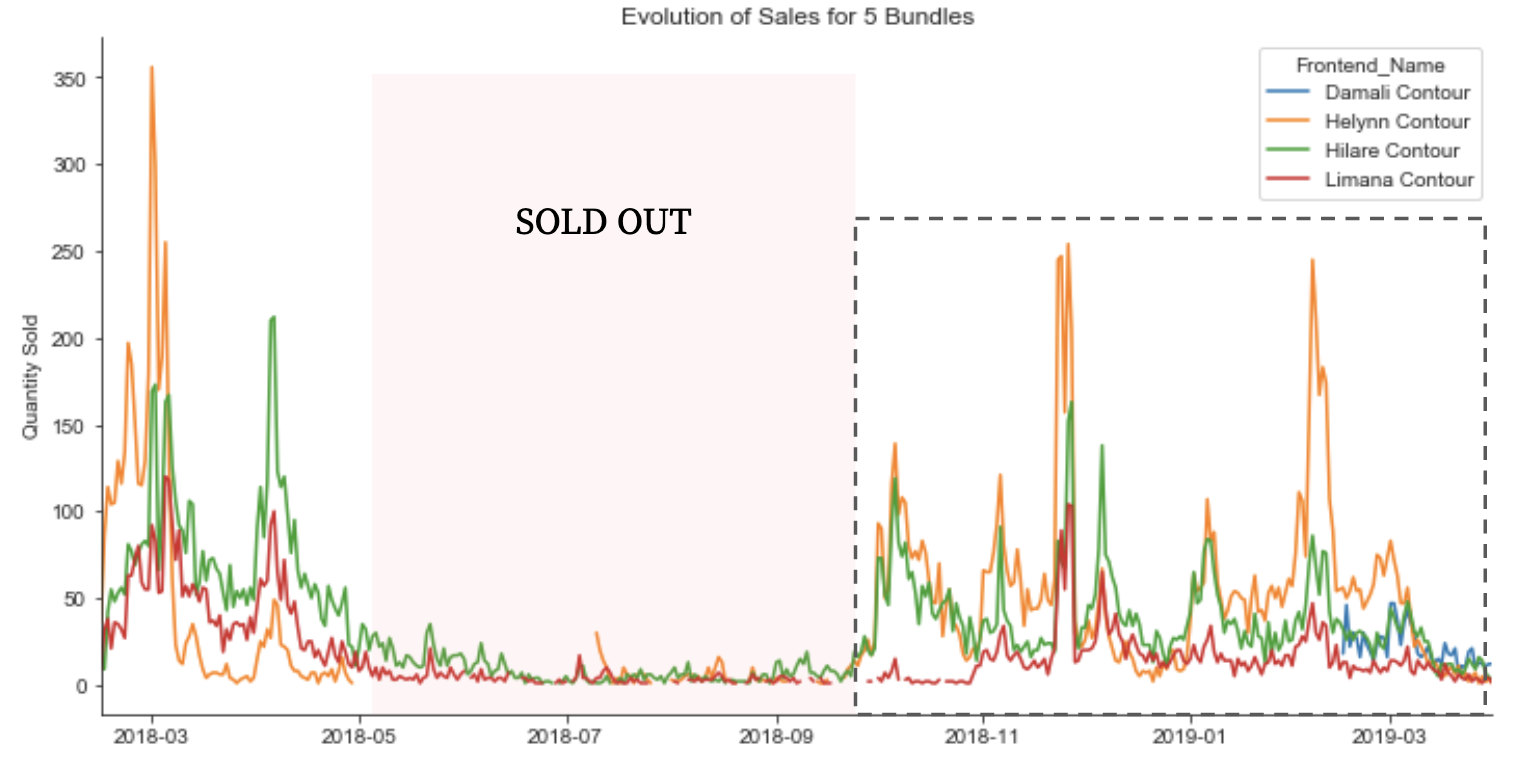
\includegraphics[width=0.8\textwidth]{graphics/evolution_3.png}%
	\caption{Evolution of sales for some sample products. Treatment of out-of-stock situations becomes critical for smooth operations, but sometimes it is wanted and \textbf{intended} outcome. Again, some products have very similar patterns of evolution and can be thought as substitutes: when one goes out of stock, a share of sales goes to another. \\
		\textit{\textbf{Data Source:} Adore Me, \textbf{Processing:} Own processing and design}}
\end{figure}


A fundamental characteristic which a model should have is robustness \cite{luca13}, and a prerequisite for choosing suitable models is a careful analysis of demand characteristics, as I have done in this paper. Researchers have highlighted some of these features: high impulse purchasing, high volatility [7], nonstationarity, uncertainty, fragmented demand across product variety, smoothness, intermittence [6], lumpiness (big spikes, long periods with zero sales), slow moving items. 

There is evidence in literature that a big challenge is estimating non-smooth demand and that traditional methods are not appropriate [8], reason why a set of new approaches has been developed: Poisson-based models [9], Binomial-based [10], Croston's model for intermittent demand [11] [12], bootstrap methods. Another essential feature is nonlinearity, for which neural networks and hierarchical models are well equiped to deal with. However, it is not a silver bullet because of training difficulties, data limitations and risk of overfitting terribly. Bartezzaghi [13] captures main causes for lumpiness and intermittence: a lot of potential (heterogeneous) clients, which might be driven by a marketing campaign, having different responses to stimuli. Adore Me actually follows some of his recommendations to reduce uncertainty: early/test sales or launches. An extremely interesting and fresh idea, is to use customer preferences presented in section 2 to anticipate lumpy and intermittent demand.



%%%%%%%%%%%%%%%%%%%%%%%%%%%%%%%%%%%%%%%%%%%%%%%%%%%%%
\subsection{Forecasting Long History Products}

\begin{figure}[!ht]
	\centering
	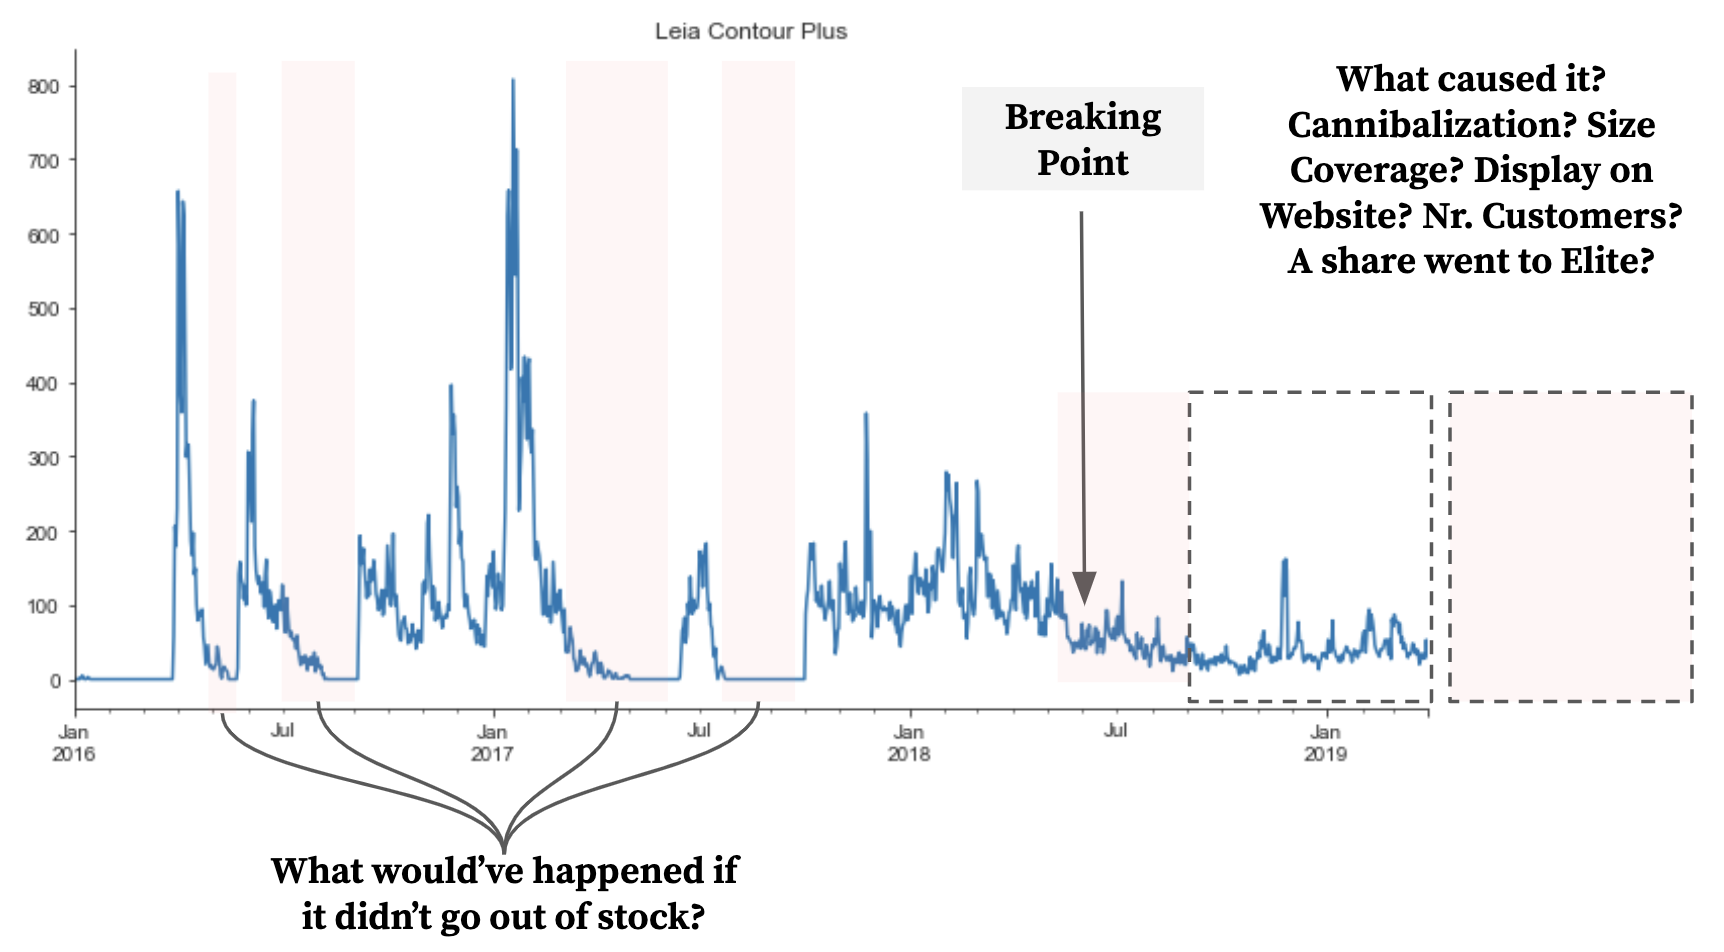
\includegraphics[width=0.8\textwidth]{graphics/evolution_1.png}%
	\caption{One of the hardest things to forecast is breaking points and changes induced by product lifecycle. The only chance we have at capturing such patterns is to step outside the ``demand management bubble``, talk to other teams and try to figure out a way to integrate external information into models and decisions we make regarding inventory. \\
		\textit{\textbf{Data Source:} Adore Me, \textbf{Processing:} Own processing and design}}
\end{figure}

Finally, I enter into a realm where we have one and a half or more years of historical data. On the one hand, I get a sense of trends, seasonality, heteroskedasticity, nonlinearity and nonstationarity. These pose a challenge, but there are well known methods to deal with these issues, however a more complicated problem, is the changing business reality and customer preferences. 

Business changes might inform an useful strategy: to heavily discount data which is ``too old``, once the pattern stabilizes either because of policies and improved processes or driven by customers. Ironically, as we strive for more data and longer histories, in fast fashion it might not improve the results much, or even be detrimental for a good forecast. Looking at the following ``trademark`` product from Adore Me, it is clear through what stages and organizational transformations the business went. In order to understand it, we need to disentangle the following effects: what products do new vs existing customers prefer, at what stage of the lifecycle is the product at, is it getting replaced by products which are more recent? Another interesting question is what would've happened if the product did not go out of stock? We can make a pretty good guess (of course using a model), given all the information that is known about the business.


\phantom{
	\cite{bater99}, \cite{brown01}, \cite{john96}, \cite{lee02}, \cite{luca13}, \cite{wang05}, \cite{soni10}
}






\newpage
%%%%%%%%%%%%%%%%%%%%%%%%%%%%%%%%%%%%%%%%%%%%%%%%%%%%%


%%%%%%%%%%%%%%%%%%%%%%%%%%%%%%%%%%%%%%%%%%%%%%%%%%%%%

%%%%%%%%%%%%%%%%%%%%%%%%%%%%%%%%%%%%%%%%%%%%%%%%%%%%%
% Conclusions %%%%%%%%%%%%%%%%%%%%%%%%%%%%%%%%%%%%%%%
%%%%%%%%%%%%%%%%%%%%%%%%%%%%%%%%%%%%%%%%%%%%%%%%%%%%%
\section{Conclusions}

In this project I put the machine learning, statistical and time series models used at Adore Me in its organizational context. Challenges that the firm faces need a variety of tools and perspectives, along with learning and alignment of various teams. In my time here I learned all aspects of what it takes to build successful data-driven products: from problem formulation, domain understanding, software architecture, data pipelines, analysis and modeling, operationalizing and monitoring models.


After identifying these challenges, I present some of the models I applied and are used at Adore Me and help to improve decision making and to make life easier for various teams. Here is a summary of main findings and things learned:

\begin{enumerate}
	\item \textbf{A content based filtering} is a simple, but appropriate method to infer customer preference and make recommendations based on it, can encode business logic and is highly interpretable. Often people disregard it in favor of Collaborative Filtering, even when their data doesn't allow the latter to work well.
	\item \textbf{Association rule mining} and Apriori algorithm is an old, but useful model to identify items which are often bought together, and can suggest improvements for merchadising team.
	\item Machine learning models used to estimate  the propensity to repurchase or unsubscribe have many more pitfalls and nuances than usually discussed in literature, related to their operationalization and generalization (in time).
	\item Sometimes, a simple A/B test is not enough in order to estimate the business impact of a targeting strategy. I suggest the method developed by Eva Ascarza to rigorously test the recommendation of propensity models.
	\item The key to demand forecasting is understanding the business dynamics and customer preferences, having clean data and designing meaningful features. A key requirement for models is stability and automation. 
	\item Classical time series analysis is very limited for Adore Me use cases, a reason more powerful methods are needed: clustering, Bayesian Hierarchical Models and even Recurrent Neural Networks.
\end{enumerate}


\newpage
%%%%%%%%%%%%%%%%%%%%%%%%%%%%%%%%%%%%%%%%%%%%%%%%%%%%%


%% BIBLIOGRAPHY ------------------------------------------
%% -------------------------------------------------------
\bibliography{bibliography}
%\bibliographystyle{apa}
	
\end{document}
